\documentclass{article}
\usepackage{amsmath}
\usepackage{amssymb}
\usepackage{graphicx}
\usepackage{hyperref}
\usepackage[version=4]{mhchem}

\title{Problem 7}
\date{}

\begin{document}
\maketitle

\section*{Problem}
In \(\triangle A B C, A B=A C=m . P\) is any point on \(B C\). Find the value of \(P A^{2}\) \(+P B \times P C\).\\
\centering
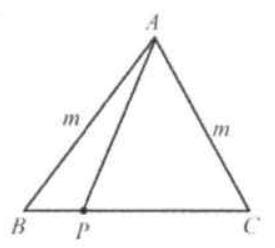
\includegraphics[width=\textwidth]{images/089(3).jpg}

\section*{Solution}
Solution not available.

\end{document}
